\chapter{Fotokimia}\label{ch:b3:photochemistry}

Penglihatan dimulai ketika satu foton membengkokkan satu molekul. Di dalam
sel-sel batang mata, retinal duduk di dalam proteinnya dalam bentuk 11-cis;
sebuah foton cahaya hijau mengubahnya menjadi bentuk all-trans, dan isomerisasi
itu praktis selesai dalam \qty{200}{fs}, lebih cepat daripada hampir semua
peristiwa kimia lain. Sisa proses penglihatan, sebuah penguatan biokimia yang
sangat besar, menyusul dari satu molekul yang bengkok itu. Aturan-aturan yang
sama (satu foton mengeksitasi satu molekul, yang lalu memilih di antara
beberapa nasib) mengatur tabir surya, sintesis cincin-cincin yang tegang,
terapi fotodinamik, asbut di atas kota-kota, dan \omterm{def:b3:photochemistry:chapman}{lapisan ozon} yang melindungi
permukaan Bumi dari cahaya ultraviolet.

\begin{recall}
\Cref{ch:b3:electronic-spectroscopy} menggambarkan keadaan-keadaan tereksitasi
molekul, \omterm{def:b3:electronic-spectroscopy:jablonski}{diagram Jablonski}, \omterm{def:b3:electronic-spectroscopy:radiationless}{lintas antarsistem}, \omterm{def:b3:electronic-spectroscopy:luminescence}{fluoresensi} dan \omterm{def:b3:electronic-spectroscopy:luminescence}{fosforesensi},
pemadaman, serta \omterm{def:b3:electronic-spectroscopy:quantum-yield}{rendemen kuantum} sebuah proses fotofisika. Jilid Tahun 1
mendefinisikan radikal, homolisis, dan isomer $Z$/$E$; jilid Tahun 2 reaksi
serempak, orbital perbatasan, dan siklus katalitik.
\Cref{ch:b3:complex-kinetics} membahas \omterm{def:b3:complex-kinetics:chain}{reaksi berantai} dan keadaan tunak.
\end{recall}

\section{Cahaya sebagai pereaksi}

Dua prinsip lama mengawali bidang ini: hanya cahaya yang diserap yang dapat
menyebabkan perubahan kimia (Grotthuss dan Draper), dan setiap foton yang
diserap mengeksitasi satu molekul (Stark dan Einstein).

\begin{definition}[Fluks foton, aktinometer kimia]\label{def:b3:photochemistry:photon-flux}
Yang disebut \emph{fluks foton}\index{fluks foton} sebuah sumber cahaya adalah
banyaknya foton yang dipancarkannya per satuan waktu, sering kali dihitung
dalam mol foton (einstein) per detik. Yang disebut \emph{aktinometer
kimia}\index{aktinometer kimia} adalah reaksi fotokimia dengan \omterm{def:b3:electronic-spectroscopy:quantum-yield}{rendemen
kuantum} yang diketahui secara teliti, yang dipakai untuk mengukur fluks foton.
\end{definition}

\begin{proposition}[Hukum Stark--Einstein]\label{prop:b3:photochemistry:stark-einstein}
Pada intensitas cahaya biasa, setiap foton yang diserap mengeksitasi tepat
satu molekul; \omterm{def:b3:electronic-spectroscopy:quantum-yield}{rendemen kuantum} primer semua proses yang berawal dari keadaan
tereksitasi itu berjumlah 1.
\end{proposition}

\begin{proof}[Bukti parsial]
Bahwa satu foton diserap oleh satu molekul pada satu waktu diterima tanpa
bukti (serapan dua foton memerlukan intensitas laser berpulsa). Molekul yang
tereksitasi itu lalu lenyap melalui proses-proses orde satu yang bersaing
dengan tetapan laju $k_i$ (\cref{ch:b3:electronic-spectroscopy}): fraksi yang
menempuh jalur $i$ adalah $\Phi_i =
k_i/\sum_jk_j$, dan $\sum_i\Phi_i = 1$.
\end{proof}

\omterm{def:b3:electronic-spectroscopy:quantum-yield}{Rendemen kuantum} sebuah reaksi, yaitu banyaknya molekul yang diubah per foton
yang diserap, tidak harus mematuhi batas ini: tahap fotokimia primer dapat
memulai sebuah rantai. Campuran \ce{H2} dan \ce{Cl2} yang terpapar cahaya
bereaksi dengan \omterm{def:b3:electronic-spectroscopy:quantum-yield}{rendemen kuantum} $10^4$ atau lebih, setiap \ce{Cl2} yang
terfotolisis memulai rantai seperti rantai reaksi hidrogen--bromin dalam
\cref{ch:b3:complex-kinetics}; \omterm{def:b3:electronic-spectroscopy:quantum-yield}{rendemen kuantum} yang lebih besar dari 1 adalah
ciri sebuah rantai.

\begin{proposition}[Laju reaksi fotokimia]\label{prop:b3:photochemistry:rate}
Larutan dengan absorbans $A$ pada panjang gelombang penyinaran, yang menerima
\omterm{def:b3:photochemistry:photon-flux}{fluks foton} $I_0$ (einstein per detik), menyerap $I_{\mathrm{abs}} = I_0(1 - 10^{-A})$;
jika pereaksi menyerap seluruhnya, reaksi mengubah $v = \Phi I_{\mathrm{abs}}$ mol
per detik.
\end{proposition}

\begin{proof}
Menurut hukum Beer--Lambert, fluks yang diteruskan adalah $I_010^{-A}$, sehingga
fluks yang diserap adalah $I_0(1 - 10^{-A})$; menurut definisi \omterm{def:b3:electronic-spectroscopy:quantum-yield}{rendemen kuantum},
$\Phi$ molekul bereaksi per foton yang diserap.
\end{proof}

\begin{method}[Laju reaksi foto dari lampunya]\label{met:b3:photochemistry:photochemical-rate}
\begin{enumerate}
  \item Energi foton $E = hc/\lambda$; \omterm{def:b3:photochemistry:photon-flux}{fluks foton} $I_0 = P/E$ untuk daya $P$
        yang mencapai sampel, atau diukur dengan aktinometer; bagilah dengan
        $N_A$ untuk memperoleh einstein per detik.
  \item Fraksi yang diserap $1 - 10^{-A}$, dengan $A$ pada panjang gelombang
        penyinaran (nilainya berubah ketika pereaksi terpakai).
  \item Laju $\Phi I_{\mathrm{abs}}$ dalam mol/s, dibagi volume untuk laju
        konsentrasi.
\end{enumerate}
\end{method}

\begin{method}[Aktinometri ferioksalat]\label{met:b3:photochemistry:actinometry}
\begin{enumerate}
  \item Sinarilah, dalam sel dan geometri yang sama dengan eksperimennya,
        larutan kalium tris(oksalato)ferat(III) yang diasamkan, cukup pekat
        untuk menyerap praktis seluruh cahaya di bawah sekitar \qty{450}{nm}.
  \item Cahaya mereduksi Fe(III) menjadi Fe(II) dengan \omterm{def:b3:electronic-spectroscopy:quantum-yield}{rendemen kuantum} yang
        terkalibrasi; setelah waktu yang terukur, tambahkan 1,10-fenantrolina
        dan bufer, lalu ukurlah absorbans kompleks merah $\ce{[Fe(phen)3]^{2+}}$.
  \item Mol Fe(II) dibagi (\omterm{def:b3:electronic-spectroscopy:quantum-yield}{rendemen kuantum} $\times$ waktu) memberikan \omterm{def:b3:photochemistry:photon-flux}{fluks
        fotonnya}.
\end{enumerate}
\end{method}

\section{Reaksi-reaksi fotokimia}

\begin{definition}[Fotoisomerisasi, keadaan fotostasioner]\label{def:b3:photochemistry:photoisomerisation}
Yang disebut \emph{fotoisomerisasi}\index{fotoisomerisasi} adalah perubahan
satu isomer menjadi isomer lain yang diinduksi cahaya, biasanya $E \to Z$
terhadap sebuah ikatan rangkap. Di bawah penyinaran terus-menerus, dua isomer
yang sama-sama menyerap mencapai \emph{keadaan
fotostasioner}\index{keadaan fotostasioner}, yaitu komposisi tunak yang
ditetapkan oleh cahaya, bukan oleh termodinamika.
\end{definition}

Puntiran ikatan rangkap menjelaskan mengapa cahaya mengisomerisasi alkena.
Dalam keadaan dasar, energi naik ketika kedua ujungnya terpuntir, sampai
maksimum pada $90^\circ$, tempat ikatan $\pi$ putus. Dalam keadaan tereksitasi
$\pi\pi^*$ urutannya terbalik: geometri terpuntir adalah yang paling stabil.
Molekul yang tereksitasi terpuntir menuju $90^\circ$, tempat kedua permukaan
saling mendekat, menyeberang kembali ke keadaan dasar di sana, lalu jatuh ke
salah satu sisi: ke isomer asalnya atau ke isomer yang lain.

\begin{omfigure}
\begin{tikzpicture}[font=\small, >=Stealth, x=0.032cm, y=1.1cm]
  \draw[->] (0,0) -- (195,0);
  \node[anchor=north] at (135,-0.45) {sudut puntiran};
  \draw[->] (0,0) -- (0,5.2) node[anchor=south] {energi};
  \foreach \t/\l in {0/{0^\circ}, 90/{90^\circ}, 180/{180^\circ}}{
    \draw (\t,0) -- (\t,-0.08) node[anchor=north] {$\l$};}
  \draw[thick, black, domain=0:180, samples=90] plot (\x,{2.6*sin(\x)^2 + 0.15*(1-cos(\x))/2});
  \draw[thick, omThm, domain=0:180, samples=90] plot (\x,{4.5 - 1.6*sin(\x)^2 + 0.1*(1-cos(\x))/2});
  \node[anchor=east] at (0,0.15) {$E$};
  \node[anchor=west] at (182,0.2) {$Z$};
  \node[omThm, anchor=south west] at (5,4.55) {$\mathrm S_1$ ($\pi\pi^*$)};
  \node[anchor=north west] at (52,1.2) {$\mathrm S_0$};
  \draw[->, omDef, thick] (12,0.12) -- (12,4.4) node[midway, left] {$h\nu$};
  \draw[->, omDef, thick, decorate, decoration={snake, amplitude=0.6mm, segment length=3mm}] (16,4.4) -- (80,3.05);
  \draw[->, omDef, thick] (90,2.85) -- (90,2.75);
  \draw[->, black!60, thick, domain=96:168, samples=40] plot (\x,{2.6*sin(\x)^2 + 0.15*(1-cos(\x))/2 + 0.28});
  \draw[->, black!60, thick, domain=84:12, samples=40] plot (\x,{2.6*sin(\x)^2 + 0.15*(1-cos(\x))/2 + 0.28});
  \node[font=\scriptsize, anchor=south, align=center] at (90,3.05) {corong};
\end{tikzpicture}

{\small Keadaan dasar ($\mathrm S_0$) dan keadaan tereksitasi pertama ($\mathrm S_1$)
sebuah alkena terhadap puntiran ikatan rangkapnya (skematis). Eksitasi isomer
$E$ (panah vertikal) diikuti puntiran pada $\mathrm S_1$ ke geometri tegak lurus,
tempat kedua permukaan hampir bersentuhan; molekul kembali ke $\mathrm S_0$ di
sana dan berelaksasi ke $E$ atau ke
$Z$.}
\end{omfigure}

\begin{proposition}[Komposisi fotostasioner]\label{prop:b3:photochemistry:pss}
Di bawah penyinaran monokromatik larutan yang tipis secara optis, dua isomer
$E$ dan $Z$ dengan koefisien absorpsi $\varepsilon_E$, $\varepsilon_Z$ dan \omterm{def:b3:electronic-spectroscopy:quantum-yield}{rendemen
kuantum} $\Phi_{E\to Z}$, $\Phi_{Z\to E}$ mencapai rasio fotostasioner
\[
  \frac{[Z]}{[E]} = \frac{\varepsilon_E\Phi_{E\to Z}}{\varepsilon_Z\Phi_{Z\to E}} .
\]
\end{proposition}

\begin{proof}
Dalam sampel yang tipis secara optis, setiap isomer menyerap fluks yang
sebanding dengan $\varepsilon[\cdot]$, sehingga
$\dd[Z]/\dd t = c(\varepsilon_E\Phi_{E\to Z}[E] - \varepsilon_Z\Phi_{Z\to E}[Z])$ dengan tetapan $c$ yang
ditentukan oleh cahaya; keadaan tunak membuat suku dalam kurung sama dengan
nol. (Hasil ini juga berlaku untuk sampel yang tebal, karena kedua isomer lalu
berbagi cahaya yang diserap dengan proporsi yang sama.)
\end{proof}

\begin{omfigure}
\begin{tikzpicture}
\begin{axis}[width=0.7\linewidth, height=5.0cm, xmin=0, xmax=120, ymin=0, ymax=1,
  axis lines=left, xlabel={waktu penyinaran / s}, ylabel={fraksi $Z$},
  tick label style={font=\small}, label style={font=\small}]
\addplot[omDef, very thick] table[x=t, y=Z] {figdata/out/bachelor-3-photostationary.dat};
\draw[black!35, densely dotted] (axis cs:0,0.801) -- (axis cs:60,0.801);
\draw[black!35, densely dotted] (axis cs:60,0.161) -- (axis cs:120,0.161);
\draw[black!35] (axis cs:60,0) -- (axis cs:60,1);
\node[font=\scriptsize, anchor=north] at (axis cs:30,0.98) {\qty{365}{nm}};
\node[font=\scriptsize, anchor=north] at (axis cs:90,0.98) {\qty{440}{nm}};
\node[font=\scriptsize, anchor=south east] at (axis cs:58,0.81) {pss 0.80};
\node[font=\scriptsize, anchor=south east] at (axis cs:118,0.17) {pss 0.16};
\end{axis}
\end{tikzpicture}

{\small Sebuah sakelar foto model (molekul mirip azobenzena) yang disinari pada
\qty{365}{nm}, tempat isomer $E$ menyerap jauh lebih kuat, lalu pada
\qty{440}{nm}, tempat isomer $Z$ yang menyerap lebih kuat: komposisinya
berpindah-pindah antara dua \omterm{def:b3:photochemistry:photoisomerisation}{keadaan fotostasioner} (pss; koefisien absorpsi dan
\omterm{def:b3:electronic-spectroscopy:quantum-yield}{rendemen kuantum} model).}
\end{omfigure}

Isomerisasi 11-cis menjadi all-trans retinal dalam rodopsin adalah reaksi
semacam itu, yang dibuat luar biasa cepat dan selektif oleh proteinnya.
Sakelar-sakelar foto sintetis yang dibangun dari azobenzena atau stilbena
dipakai untuk mengendalikan mesin molekuler, material, dan, jika dipasangkan
pada obat atau kanal ion, aktivitas biologis dengan cahaya.

\begin{definition}[Fotolisis]\label{def:b3:photochemistry:photolysis}
Yang disebut \emph{fotolisis}\index{fotolisis} adalah pemutusan ikatan oleh
cahaya. Di atmosfer, tetapan laju orde satu $j$ fotolisis sebuah spesies, yang
disebut \emph{tetapan laju fotolisis}\index{tetapan laju fotolisis} spesies itu,
menjumlahkan atas panjang gelombang hasil kali \omterm{def:b3:photochemistry:photon-flux}{fluks foton} matahari,
penampang serapan, dan \omterm{def:b3:electronic-spectroscopy:quantum-yield}{rendemen kuantum}.
\end{definition}

Sebuah foton hanya memutus ikatan jika energinya melebihi energi disosiasi:
$\lambda < hcN_A/D_0$. Untuk \ce{O2}, $D_0 = 2\Delta_fH^\circ_0(\ce{O}) = \qty{493.6}{kJ/mol}$ dari
tabel termokimia, dan hanya cahaya yang lebih pendek dari \qty{242}{nm} yang
dapat memecahnya.

Keton dan alkena yang tereksitasi juga membentuk ikatan. Dua alkena, salah
satunya tereksitasi, bergabung menjadi siklobutana: inilah fotosikloadisi
$[2+2]$, yang terlarang dalam keadaan dasar dan diizinkan dalam keadaan
tereksitasi karena alasan orbital yang diberikan dalam \cref{ch:b3:pericyclic}.
Reaksi ini membuat cincin beranggota empat, yang tegang dan sulit dicapai
dengan cara lain, dalam satu langkah.

\begin{definition}[Reaksi Norrish]\label{def:b3:photochemistry:norrish}
Yang disebut \emph{reaksi Norrish tipe I}\index{reaksi Norrish tipe I} adalah
pemutusan, oleh keton yang tereksitasi, ikatan antara karbon karbonil dan
karbon $\alpha$, menjadi radikal asil dan radikal alkil. Yang disebut
\emph{reaksi Norrish tipe II}\index{reaksi Norrish tipe II} adalah abstraksi
sebuah atom hidrogen dari karbon $\gamma$ oleh oksigen keton yang tereksitasi,
yang menghasilkan 1,4-biradikal yang terpecah menjadi enol dan alkena atau
menutup menjadi siklobutanol.
\end{definition}

\begin{omfigure}
\setchemfig{atom sep=1.9em}
\schemestart
\chemfig{H_3C-[:30]C(=[:90]O)-[:-30]CH_2-[:30]CH_2-[:-30]CH_2-[:30]CH_3}
\arrow{->[$h\nu$][via $\mathrm T_1$]}
\chemfig{H_3C-[:30]\chembelow{C}{\scriptstyle\bullet}(-[:90]OH)-[:-30]CH_2-[:30]CH_2-[:-30]\chemabove{C}{\scriptstyle\bullet}H-[:30]CH_3}
\schemestop

\medskip
\schemestart
\arrow{->[pemutusan]}[,1.1]
\chemfig{H_3C-[:30]C(-[:90]OH)=[:-30]CH_2}
\+
\chemfig{H_2C=[:30]CH-[:-30]CH_3}
\schemestop
\hspace{2.5em}
\schemestart
\arrow{->[penutupan][cincin]}[,1.1]
\chemfig{*4(-(-[::-40]OH)(-[::40]CH_3)-(-CH_3)---)}
\schemestop
\par\medskip

{\small \omterm{def:b3:photochemistry:norrish}{Reaksi Norrish tipe II} heksan-2-on. Keton triplet mengabstraksi sebuah
hidrogen dari karbon $\gamma$ melalui susunan beranggota enam; 1,4-biradikalnya
terpecah menjadi enol aseton (yang bertautomerisasi menjadi aseton) dan
propena, atau menutup menjadi 1,2-dimetilsiklobutan-1-ol.}
\end{omfigure}

Fotoreduksi benzofenon adalah versi bimolekuler yang klasik: tripletnya
mengabstraksi sebuah atom hidrogen dari pelarut alkohol seperti propan-2-ol,
dan dua radikal difenilhidroksimetil yang terbentuk bergabung menjadi
benzopinakol, yang mengkristal dari larutan.

\section{Fotosensitisasi}

\begin{definition}[Fotosensitisasi, oksigen singlet]\label{def:b3:photochemistry:sensitisation}
Yang disebut \emph{fotosensitizer}\index{fotosensitizer} adalah molekul yang
menyerap cahaya dan memindahkan energinya atau sebuah elektron ke molekul lain,
yang tidak menyerap sendiri: inilah \emph{fotosensitisasi}\index{fotosensitisasi}.
Dalam \emph{transfer energi triplet}\index{transfer energi triplet}, \omterm{def:b3:many-electron-atoms:singlet-triplet}{keadaan
triplet} sensitizer, yang terbentuk melalui \omterm{def:b3:electronic-spectroscopy:radiationless}{lintas antarsistem}, memberikan
energinya kepada akseptor saat bersentuhan, sehingga akseptor berada dalam
\omterm{def:b3:many-electron-atoms:singlet-triplet}{keadaan tripletnya}. Yang disebut \emph{oksigen singlet}\index{oksigen singlet}
adalah keadaan tereksitasi terendah \ce{O2}, ${}^1\Delta_g$, yang terbentuk dengan
cara ini dari oksigen keadaan dasar ${}^3\Sigma_g^-$.
\end{definition}

\begin{proposition}[Syarat energi untuk transfer triplet]\label{prop:b3:photochemistry:sensitisation-condition}
Transfer energi triplet--triplet dari donor D ke akseptor A berlangsung dekat
batas difusi jika $E_{\mathrm T}(\mathrm D)$ melebihi $E_{\mathrm T}(\mathrm A)$ lebih dari
sekitar \qty{10}{kJ/mol}, dan turun tajam ketika selisihnya menjadi negatif.
\end{proposition}

\begin{proof}[Bukti parsial]
Transfer ${}^3\mathrm D + \mathrm A \to \mathrm D + {}^3\mathrm A$ mempertahankan spin (dua triplet
dipertukarkan dengan satu singlet dan satu triplet) dan memerlukan
persentuhan orbital (mekanisme pertukaran, diterima tanpa bukti). Tetapan
kesetimbangannya adalah $\exp[(E_{\mathrm T}(\mathrm D) - E_{\mathrm T}(\mathrm A))/RT]$, sekitar 60 untuk
kelebihan \qty{10}{kJ/mol} pada \qty{298}{K}: tahap maju lalu terjadi pada hampir
setiap pertemuan. Jika selisihnya negatif, tetapan laju maju sama dengan batas
difusi dikalikan kebalikan faktor itu (arah yang mendaki membayar faktor
Boltzmann); kurva kuantitatifnya diterima tanpa bukti.
\end{proof}

Sensitizer yang baik menyerap di tempat akseptor tidak menyerap, berpindah ke
tripletnya dengan rendemen tinggi, dan mempunyai umur triplet yang panjang:
benzofenon, dengan rendemen triplet mendekati 1, adalah standarnya. \omterm{def:b3:photochemistry:sensitisation}{Oksigen
singlet} adalah elektrofil yang reaktif: \omterm{def:b3:photochemistry:sensitisation}{oksigen singlet} mengadisi diena dan
alkena yang kaya elektron. Dalam terapi fotodinamik, sensitizer yang
terkumpul dalam tumor, yang disinari melalui serat optik, membentuk \omterm{def:b3:photochemistry:sensitisation}{oksigen
singlet} yang menghancurkan sel-sel di sekitarnya.

\begin{definition}[Katalisis fotoredoks]\label{def:b3:photochemistry:photoredox}
Yang disebut \emph{katalisis fotoredoks}\index{katalisis fotoredoks} adalah
katalisis yang memakai \omterm{def:b3:photochemistry:sensitisation}{fotosensitizer} yang keadaan tereksitasinya sekaligus
merupakan oksidator dan reduktor yang lebih kuat daripada keadaan dasarnya
untuk memindahkan elektron tunggal ke atau dari substrat, sehingga
menghasilkan radikal di bawah cahaya tampak; sensitizer itu dibentuk kembali
dalam sebuah siklus katalitik.
\end{definition}

Kompleks rutenium $\ce{[Ru(bpy)3]^{2+}}$ adalah prototipenya: keadaan tereksitasi
transfer muatan logam-ke-ligannya, yang dicapai dengan cahaya biru dan hidup
sekitar satu mikrodetik, dapat mengambil sebuah elektron dari amina atau
memberikannya kepada halida organik. Radikal-radikal yang terbentuk ikut serta
dalam reaksi pembentukan ikatan pada kondisi yang jauh lebih lunak daripada
kondisi kimia radikal klasik.

\section{Fotokimia atmosfer}

\begin{definition}[Mekanisme Chapman, lapisan ozon]\label{def:b3:photochemistry:chapman}
Yang disebut \emph{mekanisme Chapman}\index{mekanisme Chapman} adalah himpunan empat tahap
\[
  \ce{O2 ->[h\nu] 2 O}\ (j_1), \quad \mathrm{O + O_2 + M \to O_3 + M}\ (k_2), \quad
  \ce{O3 ->[h\nu] O2 + O}\ (j_3), \quad \ce{O + O3 -> 2 O2}\ (k_4).
\]
Yang disebut \emph{lapisan ozon}\index{lapisan ozon} adalah daerah stratosfer,
sekitar 15 sampai \qty{35}{km} di atas permukaan tanah, tempat reaksi-reaksi
ini mempertahankan konsentrasi ozon yang terbesar.
\end{definition}

\begin{theorem}[Keadaan tunak Chapman]\label{thm:b3:photochemistry:chapman}
Dalam \omterm{def:b3:photochemistry:chapman}{mekanisme Chapman}, O dan \ce{O3} mencapai keadaan tunak
\[
  \frac{[\ce{O}]}{[\ce{O3}]} = \frac{j_3}{k_2[\mathrm M][\ce{O2}]}, \qquad
  [\ce{O3}] = [\ce{O2}]\sqrt{\frac{j_1k_2[\mathrm M]}{j_3k_4}} .
\]
\end{theorem}

\begin{proof}
O dan \ce{O3} saling berubah dengan cepat melalui tahap 2 dan 3 (dalam
hitungan detik), jauh lebih cepat daripada pembentukan atau pemusnahannya:
dengan menganggap pertukaran cepat itu berada dalam kesetimbangan,
$k_2[\ce{O}][\ce{O2}][\mathrm M] = j_3[\ce{O3}]$, diperoleh rasionya. Jumlah keduanya,
yaitu oksigen ganjil, dibentuk oleh tahap 1 (dua O per \ce{O2}) dan dimusnahkan
oleh tahap 4 (dua oksigen ganjil per peristiwa):
$2j_1[\ce{O2}] = 2k_4[\ce{O}][\ce{O3}]$. Menyubstitusikan $[\ce{O}]$ dari rasio itu memberikan $[\ce{O3}]^2 = j_1k_2[\mathrm M][\ce{O2}]^2/(j_3k_4)$.
\end{proof}

Dengan tetapan laju dari basis data terevaluasi dan laju \omterm{def:b3:photochemistry:photolysis}{fotolisis} yang khas
pada \qty{30}{km} (data soal akhir pekan), model Chapman memberikan sekitar
$\num{6e12}$ molekul ozon per \unit{cm^3}, kira-kira lima belas bagian per juta.
Jika diintegralkan terhadap ketinggian, seluruh atmosfer memuat rata-rata
sekitar 300 satuan Dobson ozon: jika dimampatkan pada tekanan permukaan, lapisan
setebal \qty{3}{mm}. \omterm{def:b3:photochemistry:chapman}{Mekanisme Chapman} saja meramalkan ozon yang lebih banyak
daripada yang teramati: siklus-siklus katalitik memusnahkan ozon lebih cepat.

\begin{definition}[Penipisan ozon, spesies reservoir]\label{def:b3:photochemistry:ozone-depletion}
Yang disebut \emph{penipisan ozon}\index{penipisan ozon} adalah berkurangnya
kolom ozon stratosfer yang disebabkan oleh siklus-siklus katalitik radikal (Cl
dan ClO, juga NO dan \ce{NO2}, serta OH dan \ce{HO2}). Yang disebut \emph{spesies
reservoir}\index{spesies reservoir} adalah molekul stabil (HCl, \ce{ClONO2}) yang
menahan radikal katalitik dalam bentuk tidak aktif, yang darinya radikal itu
kelak dapat dilepaskan kembali.
\end{definition}

\begin{omfigure}
\begin{tikzpicture}[font=\small, >=Stealth]
  \node (cl) at (0,0) {Cl};
  \node (clo) at (3.2,0) {ClO};
  \draw[->, thick, omThm] (cl) to[bend left=40] node[midway, above] {$+\,\ce{O3}$, $-\,\ce{O2}$} (clo);
  \draw[->, thick, omThm] (clo) to[bend left=40] node[midway, below] {$+\,\ce{O}$, $-\,\ce{O2}$} (cl);
  \node[font=\scriptsize, align=center] at (1.6,0) {neto\\ $\ce{O + O3 -> 2 O2}$};
  \draw[->, black!55] (cl) -- (-1.6,-1.2) node[below, font=\scriptsize] {$+\,\ce{CH4} \to$ HCl};
  \draw[->, black!55] (clo) -- (4.8,-1.2) node[below, font=\scriptsize] {$+\,\ce{NO2} \to \ce{ClONO2}$};
  \node (o2) at (8.0,1.3) {\ce{O2}};
  \node (o) at (8.0,-1.1) {O};
  \node (o3) at (11.4,-1.1) {\ce{O3}};
  \draw[->, thick] (o2) -- (o) node[midway, left, font=\scriptsize] {$h\nu$};
  \draw[->, thick] (o.south east) to[bend right=30] node[midway, below, font=\scriptsize] {$+\,\ce{O2}$, M} (o3.south west);
  \draw[->, thick] (o3.north west) to[bend right=30] node[midway, above, font=\scriptsize] {$h\nu$} (o.north east);
  \draw[->, thick, black!55] (o3.north) -- (o2.east) node[midway, above right, font=\scriptsize] {$+\,\ce{O}$};
\end{tikzpicture}

{\small Kiri: siklus katalitik klorin, yang memusnahkan satu molekul ozon dan
satu atom oksigen pada setiap putaran dan mengembalikan atom klorinnya; panah
kelabu menuju ke reservoir. Kanan: siklus Chapman, tempat \ce{O} dan \ce{O3}
bertukar dengan cepat melalui rekombinasi dan \omterm{def:b3:photochemistry:photolysis}{fotolisis} sementara tahap-tahap
yang lambat membentuk dan memusnahkan oksigen ganjil.}
\end{omfigure}

\begin{proposition}[Panjang rantai siklus klorin]\label{prop:b3:photochemistry:catalytic-destruction}
Jika pada setiap putaran atom Cl bereaksi dengan \ce{O3} dengan peluang $p_1 =
k[\ce{O3}]/(k[\ce{O3}] + k'[\ce{CH4}])$ dan radikal ClO dengan O dengan peluang $p_2 =
k''[\ce{O}]/(k''[\ce{O}] + k'''[\ce{NO2}])$, banyaknya putaran rata-rata sebelum klorin
tertangkap dalam reservoir adalah $p/(1 - p)$ dengan $p = p_1p_2$; setiap
putaran memusnahkan satu molekul ozon.
\end{proposition}

\begin{proof}
Setiap putaran diselesaikan dengan peluang $p$, tidak bergantung pada
putaran-putaran sebelumnya: banyaknya putaran $n$ yang selesai sebelum
penangkapan mempunyai peluang $p^n(1 -
p)$, dan $\sum_nnp^n(1 - p) = p/(1 - p)$.
\end{proof}

\begin{omfigure}
\begin{tikzpicture}
\begin{axis}[name=oc, width=0.47\linewidth, height=5.2cm, xmin=0, xmax=120, ymin=0, ymax=6.4,
  axis lines=left, xlabel={waktu / hari}, ylabel={$[\ce{O3}]$ / $10^{12}$ \unit{cm^{-3}}},
  tick label style={font=\small}, label style={font=\small},
  legend style={font=\scriptsize, draw=none, fill=white, fill opacity=0.85, text opacity=1,
  at={(0.97,0.03)}, anchor=south east}, legend cell align=left, title={\small stratosfer}]
\addplot[black, thick] table[x=day, y=noCl] {figdata/out/bachelor-3-ozone-chemistry-chapman.dat};
\addplot[omDef, thick] table[x=day, y=Cl1] {figdata/out/bachelor-3-ozone-chemistry-chapman.dat};
\addplot[omThm, thick] table[x=day, y=Cl3] {figdata/out/bachelor-3-ozone-chemistry-chapman.dat};
\legend{Chapman, $+$ \qty{1e7}{cm^{-3}} ClO$_x$, $+$ \qty{3e7}{cm^{-3}} ClO$_x$}
\end{axis}
\begin{axis}[at={(oc.east)}, anchor=west, xshift=1.5cm, width=0.47\linewidth, height=5.2cm,
  xmin=0, xmax=4, ymin=0, ymax=80, axis lines=left, xlabel={$[\ce{NO2}]/[\ce{NO}]$},
  ylabel={$[\ce{O3}]$ / ppb}, tick label style={font=\small}, label style={font=\small},
  title={\small udara tercemar pada tengah hari}]
\addplot[omDef, very thick] table[x=ratio, y=O3ppb] {figdata/out/bachelor-3-ozone-chemistry-leighton.dat};
\end{axis}
\end{tikzpicture}

{\small Kiri: ozon pada ketinggian model sekitar \qty{30}{km} (\qty{230}{K},
tetapan laju terevaluasi, laju \omterm{def:b3:photochemistry:photolysis}{fotolisis} soal akhir pekan), yang terbentuk
mulai dari nol menurut \omterm{def:b3:photochemistry:chapman}{mekanisme Chapman}, dan lebih rendah dengan adanya
siklus klorin. Kanan: \omterm{def:b3:photochemistry:photoisomerisation}{keadaan fotostasioner} Leighton udara tercemar pada
\qty{298}{K}, $[\ce{O3}] = j[\ce{NO2}]/k[\ce{NO}]$ dengan $j = \qty{8e-3}{s^{-1}}$ (nilai
model pada tengah hari).}
\end{omfigure}

Setiap atom klorin, yang dibebaskan di stratosfer dari klorofluorokarbon oleh
\omterm{def:b3:photochemistry:photolysis}{fotolisis} ultraviolet, memusnahkan ozon dalam puluhan putaran sebelum
tersimpan sebagai HCl atau \ce{ClONO2}, dan dilepaskan kembali berkali-kali
selama bertahun-tahun ia berada di sana. Di atas Antarktika, selama malam
kutub, terbentuk awan es dan hidrat asam nitrat; pada permukaannya kedua
reservoir itu bereaksi satu sama lain, $\ce{HCl + ClONO2 -> Cl2 + HNO3}$, asam
nitratnya tetap berada di dalam partikel, dan ketika Matahari kembali pada
musim semi \ce{Cl2} terfotolisis: karena \ce{NO2} telah tersingkir, klorin itu
tidak tertangkap kembali, dan sebuah siklus melalui dimer ClO memusnahkan
ozon tanpa memerlukan atom O. Kolom ozon turun menjadi sekitar 100 satuan
Dobson: inilah lubang ozon.

\begin{proposition}[Hubungan Leighton]\label{prop:b3:photochemistry:leighton}
Dalam udara yang disinari matahari, tempat ozon hanya dibentuk oleh \omterm{def:b3:photochemistry:photolysis}{fotolisis}
\ce{NO2} dan hanya dimusnahkan oleh NO, ketiga spesies itu mencapai \omterm{def:b3:photochemistry:photoisomerisation}{keadaan
fotostasioner}
\[
  [\ce{O3}] = \frac{j_{\ce{NO2}}[\ce{NO2}]}{k[\ce{NO}]} .
\]
\end{proposition}

\begin{proof}
$\ce{NO2 ->[h\nu] NO + O}$ ($j_{\ce{NO2}}$), $\mathrm{O + O_2 + M \to O_3 + M}$ (cepat: setiap atom O
membentuk satu \ce{O3}), dan
$\ce{NO + O3 -> NO2 + O2}$ ($k$): pada keadaan tunak, ozon yang dibentuk,
$j_{\ce{NO2}}[\ce{NO2}]$, sama dengan ozon yang dimusnahkan, $k[\ce{NO}][\ce{O3}]$.
\end{proof}

Siklus itu sendiri tidak membentuk ozon neto: siklus itu hanya
mempertukarkan NO, \ce{NO2} dan \ce{O3}. Yang menaikkan rasio $[\ce{NO2}]/[\ce{NO}]$, dan
karena itu ozonnya, adalah oksidasi NO menjadi \ce{NO2} tanpa memakai ozon,
oleh radikal-radikal peroksi yang berasal dari oksidasi hidrokarbon oleh OH,
sang deterjen troposfer.

\begin{definition}[Asbut fotokimia]\label{def:b3:photochemistry:smog}
Yang disebut \emph{asbut fotokimia}\index{asbut fotokimia} adalah campuran ozon,
nitrogen dioksida, aldehida, peroksiasil nitrat, dan partikel halus yang
terbentuk dalam udara bersinar matahari yang tercemar oleh nitrogen oksida
dan senyawa organik mudah menguap.
\end{definition}

\begin{omfigure}
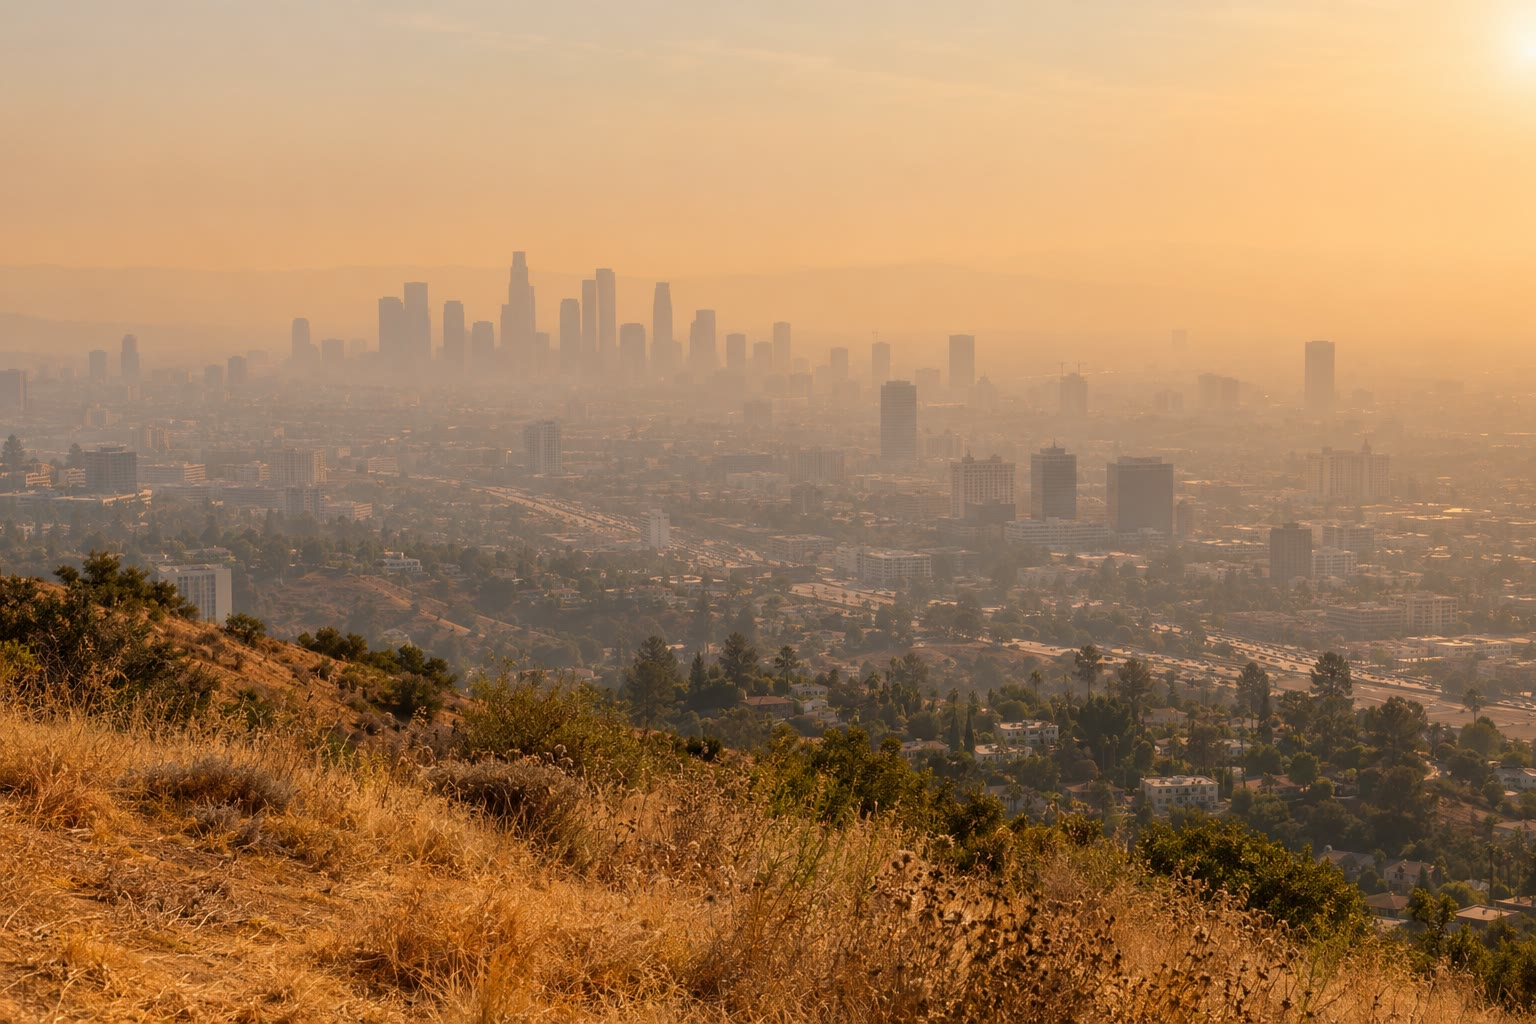
\includegraphics[width=0.6\linewidth]{images/book4/ai/b3-14-smog.jpg}

{\small Sebuah kota di bawah \omterm{def:b3:photochemistry:smog}{asbut fotokimia} pada sore hari yang panas. Warna
kecokelatannya berasal dari \ce{NO2}; ozonnya, yang mengiritasi paru-paru, tidak
terlihat.}
\end{omfigure}

\begin{omfigure}
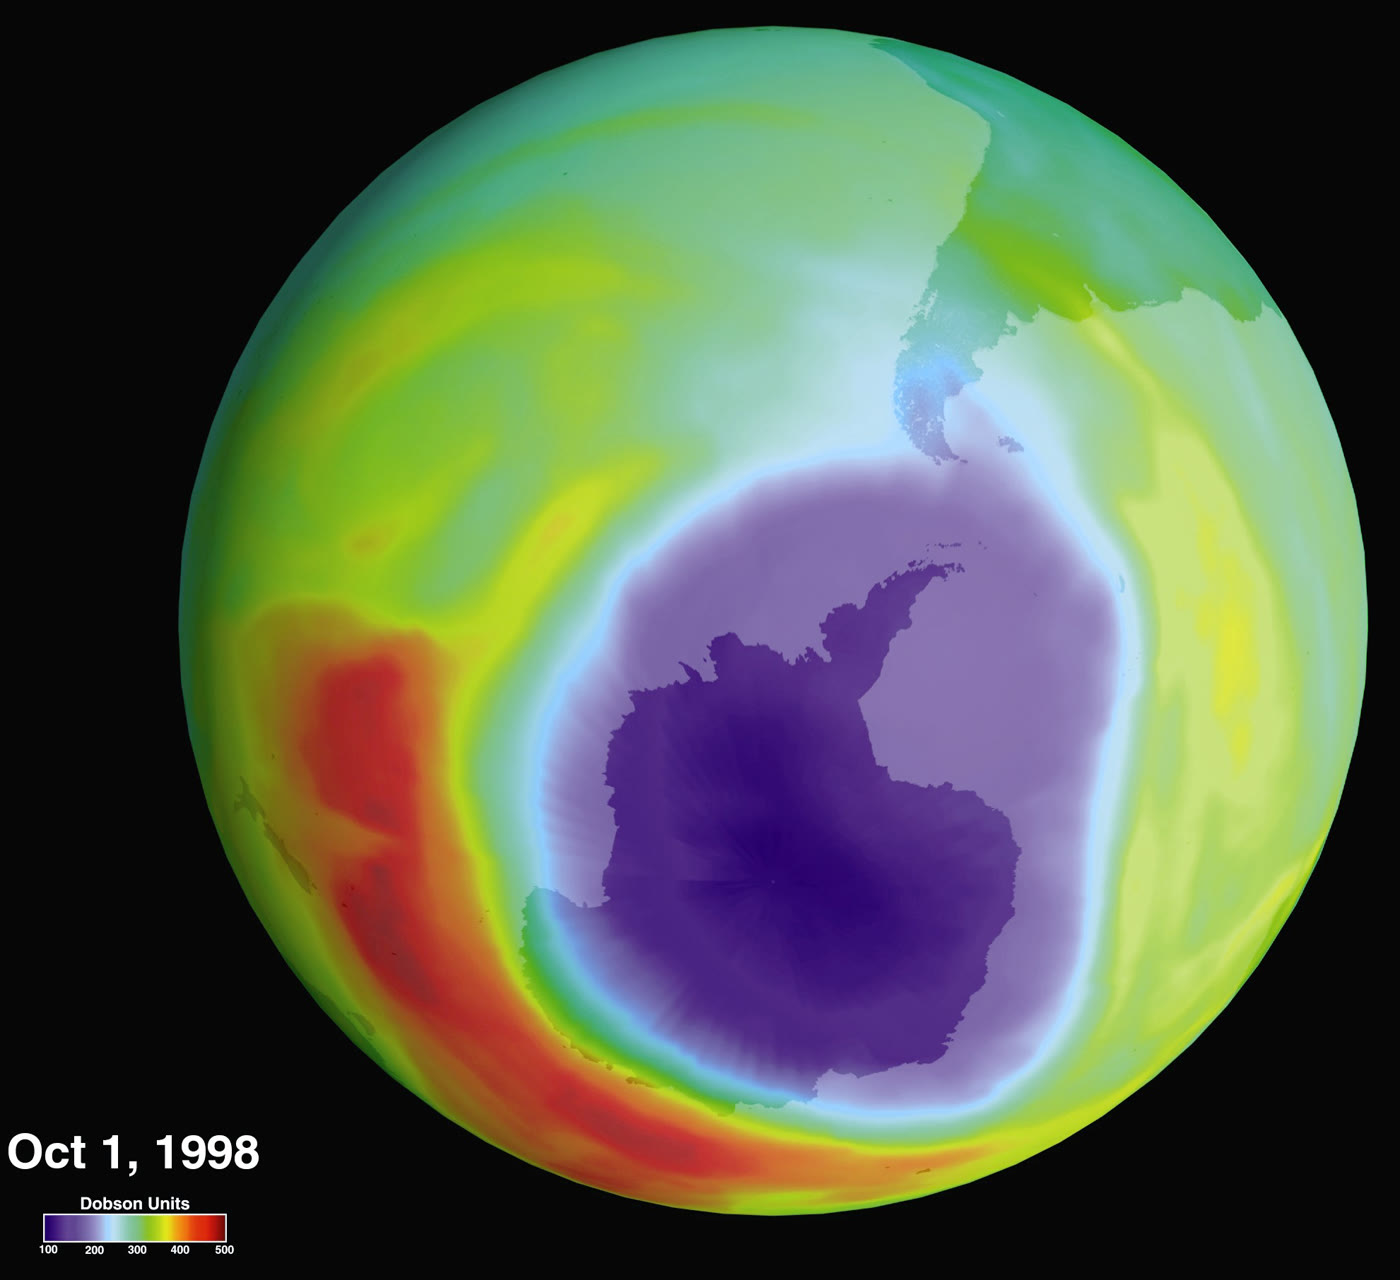
\includegraphics[width=0.5\linewidth]{images/book4/ozone-hole.jpg}

{\small Kolom ozon di atas belahan bumi selatan pada 1 Oktober 1998, dari
pengukuran satelit: lubang ozon di atas Antarktika (ungu) turun sampai sekitar
100 satuan Dobson, dibandingkan dengan sekitar 300 di tempat lain.}
\end{omfigure}

\begin{inthelab}[Sebuah fotoreaktor]
Sebuah lampu raksa bertekanan menengah, yang didinginkan dalam selubung kuarsa,
berada di tengah bejana reaksi; selubung filter kaca menyingkirkan panjang
gelombang di bawah sekitar \qty{300}{nm}, yang akan merusak produknya.
Larutannya dibebaskan dari oksigen dengan aliran nitrogen (oksigen memadamkan
triplet) dan diaduk. Seluruh reaktor tertutup: lampu itu memancarkan cahaya
ultraviolet yang berbahaya bagi mata dan kulit, dan tidak pernah dipandang,
walaupun sebentar.
\end{inthelab}

\begin{safety}{\ghs[0.8cm]{GHS08}\ghs[0.8cm]{GHS09}}
% ledger: ghs4:benzophenone
Benzofenon, sensitizer yang umum dan pereaksi fotoreduksi: diduga dapat
menyebabkan kanker, dapat merusak organ setelah paparan berkepanjangan,
beracun bagi kehidupan akuatik. Ditimbang dan ditangani dengan sarung
tangan; sisanya dibuang ke limbah organik.
\end{safety}

\begin{history}[Fotokimia masa depan, dan lubang di langit]
Pada tahun 1912 Giacomo Ciamician, di Bologna, bertanya apakah suatu hari
industri dapat berjalan dengan cahaya matahari, seperti tumbuhan, alih-alih
dengan batu bara; ia telah bertahun-tahun memaparkan labu-labu berisi senyawa
organik pada matahari di atap laboratoriumnya. Pada tahun 1985, tiga ilmuwan
yang bekerja di sebuah stasiun penelitian Antarktika melaporkan bahwa kolom
ozon musim semi di atasnya terus turun tajam sejak akhir tahun 1970-an.
Lubang ozon, yang dalam beberapa tahun dijelaskan oleh kimia dalam bab ini,
membawa pada penghapusan bertahap klorofluorokarbon.
\end{history}

\section{Latihan}

\begin{exercise}[$\star$]\label{exo:b3:photochemistry:1}
Sebuah lampu memberikan \qty{100}{mW} pada \qty{365}{nm}. Berapa banyak foton per
detik, dan berapa einstein per detik?
\end{exercise}

\begin{exercise}[$\star$]\label{exo:b3:photochemistry:2}
Dalam \qty{10.0}{min}, sebuah larutan yang menyerap
\qty{1.00e-7}{einstein.s^{-1}} mengubah \qty{2.0e-5}{mol} pereaksi. Hitunglah
\omterm{def:b3:electronic-spectroscopy:quantum-yield}{rendemen kuantumnya}.
\end{exercise}

\begin{exercise}[$\star$]\label{exo:b3:photochemistry:3}
Reaksi fotokimia \ce{H2} dengan \ce{Cl2} mempunyai \omterm{def:b3:electronic-spectroscopy:quantum-yield}{rendemen kuantum} sampai
$10^4$ atau lebih. Apa yang ditunjukkan hal ini? Tuliskan tahap-tahap
propagasinya.
\end{exercise}

\begin{exercise}[$\star$]\label{exo:b3:photochemistry:4}
% ledger: janaf:O.dfH0, janaf:O3.dfH0
Dari entalpi pembentukan pada 0 K untuk O (\qty{246.79}{kJ/mol}) dan \ce{O3}
(\qty{145.35}{kJ/mol}), hitunglah panjang gelombang terpanjang yang dapat
memecah \ce{O2} menjadi dua atom dan \ce{O3} menjadi \ce{O2} dan O.
\end{exercise}

\begin{exercise}[$\star\star$]\label{exo:b3:photochemistry:5}
Sebuah sakelar foto mempunyai, pada \qty{365}{nm}, $\varepsilon_E = 22\,000$ dan
$\varepsilon_Z = 1500$ \unit{L.mol^{-1}.cm^{-1}}, dengan $\Phi_{E\to Z} = 0.11$ dan
$\Phi_{Z\to E} = 0.40$ (data latihan). Hitunglah komposisi fotostasionernya.
\end{exercise}

\begin{exercise}[$\star\star$]\label{exo:b3:photochemistry:6}
Berikan produk-produk \omterm{def:b3:photochemistry:norrish}{reaksi Norrish tipe II} heksan-2-on, dan jelaskan mengapa
pentan-2-on memberikan etena, bukan propena.
\end{exercise}

\begin{exercise}[$\star\star$]\label{exo:b3:photochemistry:7}
Sebuah akseptor mempunyai energi triplet \qty{250}{kJ/mol}. Di antara tiga
kandidat sensitizer dengan energi triplet 289, 253 dan \qty{236}{kJ/mol} (data
latihan), manakah yang memindahkan energi secara efisien? Perkirakan tetapan
kesetimbangan transfer untuk masing-masing pada \qty{298}{K}.
\end{exercise}

\begin{exercise}[$\star\star$]\label{exo:b3:photochemistry:8}
% ledger: kin:O+O2+M.k0, kin:O+O2+M.n
Pada \qty{230}{K}, dengan $[\mathrm M] = \qty{4.0e17}{cm^{-3}}$, $[\ce{O2}] = 0.21[\mathrm M]$
dan $j_3 = \qty{1.0e-3}{s^{-1}}$, hitunglah $k_2$ dan rasio keadaan tunak
$[\ce{O}]/[\ce{O3}]$.
\end{exercise}

\begin{exercise}[$\star\star$]\label{exo:b3:photochemistry:9}
% ledger: kin:Cl+O3.A, kin:Cl+O3.EaR, kin:Cl+CH4.A, kin:Cl+CH4.EaR
Pada \qty{230}{K}, hitunglah tetapan laju $\ce{Cl + O3}$ dan $\ce{Cl + CH4}$, serta
peluang bahwa sebuah atom Cl bertemu dengan \ce{O3} dan bukan dengan \ce{CH4}
jika $[\ce{O3}] = \qty{5.7e12}{cm^{-3}}$ dan $[\ce{CH4}] = \qty{4.0e11}{cm^{-3}}$.
\end{exercise}

\begin{exercise}[$\star\star\star$]\label{exo:b3:photochemistry:10}
% ledger: kin:NO+O3.A, kin:NO+O3.EaR
Pada tengah hari di sebuah kota, $[\ce{NO2}]/[\ce{NO}] = 1.5$ dan
$j_{\ce{NO2}} = \qty{8.0e-3}{s^{-1}}$. Hitunglah ozon fotostasionernya pada
\qty{298}{K} dalam molekul per \unit{cm^3} dan dalam ppb (udara pada \qty{1}{bar}).
Apa yang terjadi pada malam hari?
\end{exercise}

\begin{exercise}[$\star\star\star$]\label{exo:b3:photochemistry:11}
Larutan \qty{3.0}{mL} dengan absorbans 0.50 pada \qty{313}{nm} menerima
\qty{50}{mW} cahaya pada panjang gelombang itu; reaksinya mempunyai
$\Phi = 0.25$. Hitunglah laju awalnya dalam \unit{mol.L^{-1}.s^{-1}}.
\end{exercise}

\begin{exercise}[$\star\star\star$]\label{exo:b3:photochemistry:12}
Sebuah aktinometer ferioksalat, dengan \omterm{def:b3:electronic-spectroscopy:quantum-yield}{rendemen kuantum} 1.25 pada
\qty{365}{nm} (data latihan) dan serapan total, membentuk \qty{3.0e-6}{mol}
Fe(II) dalam \qty{60}{s}. Hitunglah \omterm{def:b3:photochemistry:photon-flux}{fluks fotonnya}. Mengapa konversinya harus
tetap kecil?
\end{exercise}

\section{Soal: Membentuk dan Merusak Lapisan Ozon}

\begin{problem}[{Soal akhir pekan --- membentuk dan merusak lapisan ozon: ambang
energi foton, keadaan tunak Chapman dengan tetapan laju terevaluasi, siklus
klorin, dan reservoir yang menghentikannya}]
\label{pb:b3:photochemistry:1}
% ledger: janaf:O.dfH0, janaf:O3.dfH0, kin:O+O2+M.k0, kin:O+O2+M.n, kin:O+O3.A, kin:O+O3.EaR, kin:Cl+O3.A, kin:Cl+O3.EaR, kin:O+ClO.A, kin:O+ClO.EaR, kin:Cl+CH4.A, kin:Cl+CH4.EaR, kin:ClO+NO2+M.k0, kin:ClO+NO2+M.n, kin:ClO+NO2+M.kinf, kin:ClO+NO2+M.Fc, oz:column.mean, oz:column.hole
Sebuah model stratosfer di dekat \qty{30}{km} (data soal): $T = \qty{230}{K}$, $[\mathrm M] =
\qty{4.0e17}{cm^{-3}}$, $[\ce{O2}] = 0.21[\mathrm M]$, \omterm{def:b3:photochemistry:photolysis}{tetapan laju fotolisis} $j_1 = \qty{1.0e-11}{s^{-1}}$
(\ce{O2}) dan $j_3 = \qty{1.0e-3}{s^{-1}}$ (\ce{O3}), $[\ce{CH4}] = \qty{4.0e11}{cm^{-3}}$,
$[\ce{NO2}] = \qty{1.0e9}{cm^{-3}}$. Tetapan laju terevaluasi (\unit{cm^3.s^{-1}}, atau
\unit{cm^6.s^{-1}} untuk $k_2$, dengan konsentrasi dihitung per \unit{cm^3}):
$k_2 = \num{6.0e-34}(T/300)^{-2.6}$; $k_4 = \num{8.0e-12}\eu^{-2060/T}$; Cl + \ce{O3}: $\num{2.8e-11}\eu^{-250/T}$;
O + ClO: $\num{2.5e-11}\eu^{110/T}$; Cl + \ce{CH4}: $\num{6.6e-12}\eu^{-1240/T}$; ClO + \ce{NO2} + M:
$\num{1.41e-13}$ pada kondisi ini.

\medskip\noindent\textbf{Bagian I --- Ambang energi foton.}
\begin{enumerate}[beginpenalty=10000]
  \item Hitunglah $D_0(\ce{O2})$ dari $\Delta_fH^\circ_0(\ce{O}) = \qty{246.79}{kJ/mol}$.
  \item Simpulkan panjang gelombang terpanjang yang memecah \ce{O2}.
  \item Hitunglah energi $\ce{O3 -> O2 + O}$ ($\Delta_fH^\circ_0(\ce{O3}) = \qty{145.35}{kJ/mol}$)
        dan panjang gelombang ambangnya.
  \item Dengan demikian cahaya tampak dapat memecah ozon; mengapa serapan
        ultraviolet ozonlah yang penting bagi kehidupan?
  \item Mengapa \ce{O2} hanya terfotolisis di bagian atmosfer yang tinggi?
\end{enumerate}

\medskip\noindent\textbf{Bagian II --- Keadaan tunak Chapman.}
\begin{enumerate}[resume, beginpenalty=10000]
  \item Tuliskan keempat tahap Chapman.
  \item Hitunglah $k_2$ dan $k_2[\mathrm M]$ pada \qty{230}{K}.
  \item Hitunglah $k_4$.
  \item Hitunglah $[\ce{O}]/[\ce{O3}]$.
  \item Tunjukkan bahwa $[\ce{O3}] = [\ce{O2}]\sqrt{j_1k_2[\mathrm M]/(j_3k_4)}$.
  \item Hitunglah $[\ce{O3}]$ dan rasio pencampurannya.
  \item Hitunglah $[\ce{O}]$.
  \item Ozon yang teramati lebih rendah daripada nilai ini. Mengapa?
\end{enumerate}

\medskip\noindent\textbf{Bagian III --- Siklus klorin.}
\begin{enumerate}[resume, beginpenalty=10000]
  \item Tuliskan siklus itu dan reaksi netonya.
  \item Hitunglah umur atom Cl terhadap \ce{O3}.
  \item Hitunglah umur ClO terhadap O.
  \item Simpulkan rasio tunak $[\ce{ClO}]/[\ce{Cl}]$.
  \item Dengan $[\ce{Cl}] + [\ce{ClO}] = \qty{1.0e7}{cm^{-3}}$, bandingkan laju
        kehilangan oksigen ganjil oleh siklus itu dengan laju tahap Chapman
        $\ce{O + O3}$.
  \item Tahap mana yang membatasi siklus itu?
\end{enumerate}

\medskip\noindent\textbf{Bagian IV --- Reservoir.}
\begin{enumerate}[resume, beginpenalty=10000]
  \item Hitunglah peluang bahwa atom Cl bereaksi dengan \ce{O3} dan bukan dengan
        \ce{CH4}.
  \item Hitunglah peluang bahwa ClO bereaksi dengan O dan bukan dengan
        \ce{NO2}.
  \item Simpulkan peluang $p$ bahwa satu putaran siklus diselesaikan.
  \item Simpulkan banyaknya putaran rata-rata sebelum klorin itu tertangkap.
  \item Jelaskan bagaimana awan stratosfer kutub memperpanjang rantai itu.
  \item Nyatakan hasilnya: banyaknya molekul ozon yang dimusnahkan satu atom
        klorin, dalam model ini, sebelum atom itu tertangkap dalam reservoir.
\end{enumerate}
\end{problem}
